\documentclass{article}
\usepackage[final]{neurips_2020}

\usepackage[utf8]{inputenc}
\usepackage{ctex}
\usepackage[T1]{fontenc}    % use 8-bit T1 fonts
\usepackage{hyperref}       % hyperlinks
\usepackage{url}            % simple URL typesetting
\usepackage{booktabs}       % professional-quality tables
\usepackage{amsfonts}       % blackboard math symbols
\usepackage{amsmath}
\usepackage{nicefrac}       % compact symbols for 1/2, etc.
\usepackage{microtype}      % microtypography
\usepackage{indentfirst}
\usepackage{listings}
\usepackage{graphicx}
\usepackage{graphics}
\usepackage{float}
\usepackage[dvipsnames]{xcolor}
\lstset{
    language=Python, % 设置语言
    basicstyle=\ttfamily, % 设置字体族
    breaklines=true, % 自动换行
    keywordstyle=\bfseries\color{NavyBlue}, % 设置关键字为粗体,颜色为 NavyBlue
    morekeywords={}, % 设置更多的关键字,用逗号分隔
    emph={self}, % 指定强调词,如果有多个,用逗号隔开
    emphstyle=\bfseries\color{Rhodamine}, % 强调词样式设置
    commentstyle=\itshape\color{black!50!white}, % 设置注释样式,斜体,浅灰色
    stringstyle=\bfseries\color{PineGreen!90!black}, % 设置字符串样式
    columns=flexible,
    numbers=left, % 显示行号在左边
    numbersep=2em, % 设置行号的具体位置
    numberstyle=\footnotesize, % 缩小行号
    frame=single, % 边框
    framesep=1em, % 设置代码与边框的距离
    showstringspaces=false
}
\setlength{\parindent}{2em}

\title{2023 年秋季计算机体系结构——大作业\\Speculative Tomasulo算法实现}

\author{%
    21307099 李英骏\\
    \texttt{liyj323@mail2.sysu.edu.cn} \\
}

\begin{document}
\maketitle

\begin{abstract}
    Tomasulo算法的原始结构如下图(\ref{fig: rough Toma})所示
    \begin{figure}[H]
        \centering
        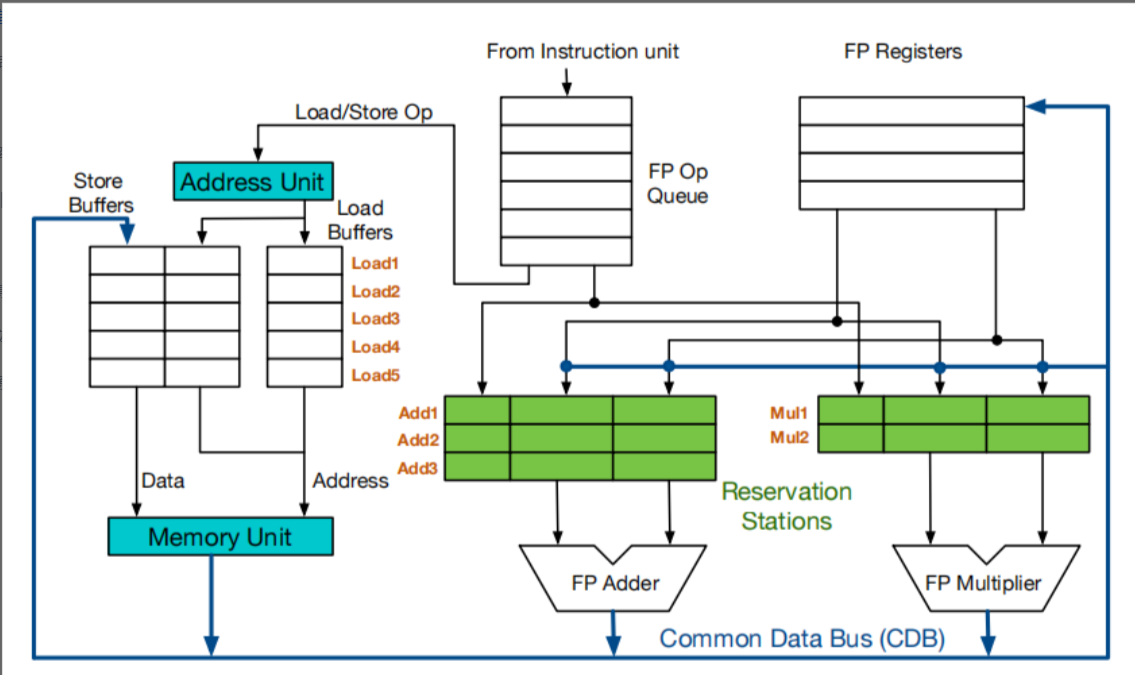
\includegraphics[width=0.9\linewidth]{Tomasulo.png}
        \caption{原始Tomasulo}
        \label{fig: rough Toma}
    \end{figure}
    其缺点在于:
    \begin{itemize}
        \item 一个周期只能写回一条指令
        \item 在多发射情形下,存储指令之间可以有数据冲突,需要额外的逻辑进行调度
        \item 不能保证按序提交,因此难以处理分支指令,也无法实现精确中断。
        \item \dots
    \end{itemize}
    因此设计人员提出了重排序缓冲的概念,利用这一概念,可以改进Tomasulo算法(如图\ref{fig: spec Toma}),
    从而实现处理器的按序发射-乱序执行-按序提交。
    \begin{figure}[H]
        \centering
        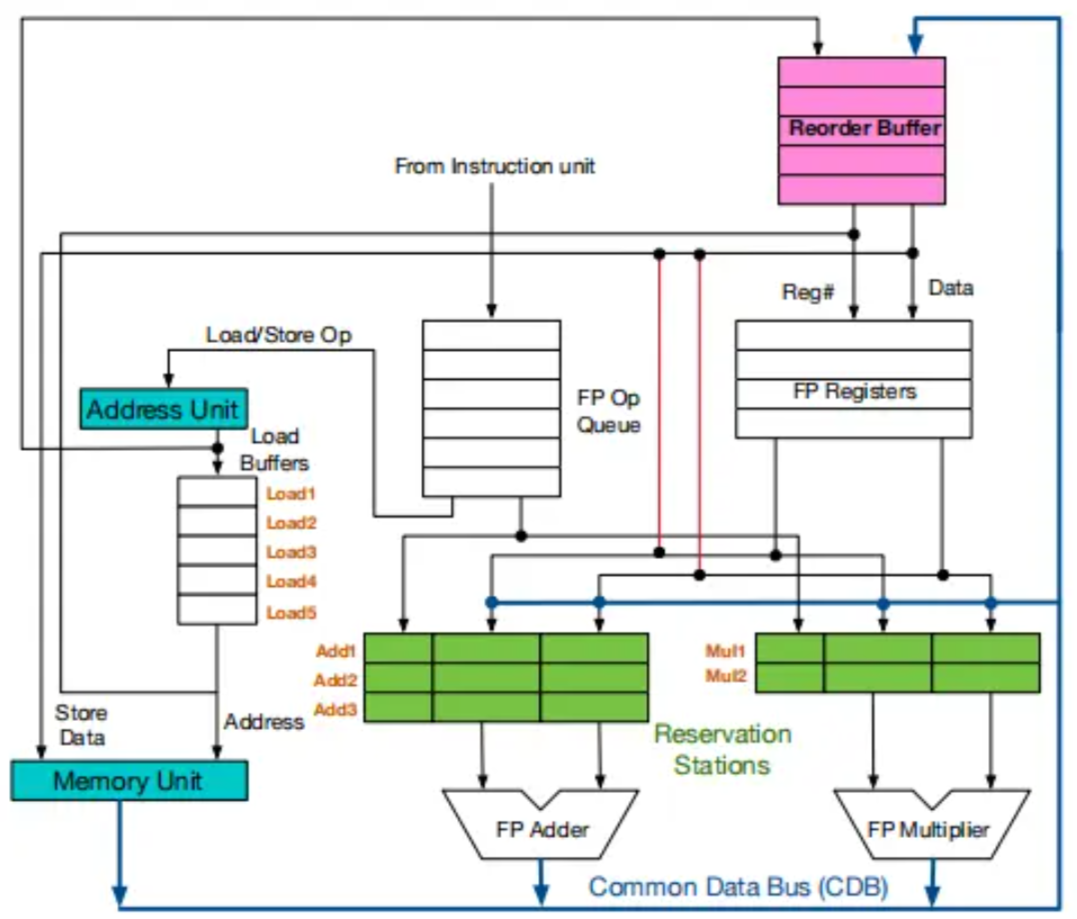
\includegraphics[width=0.9\linewidth]{Tomasulo_2.png}
        \caption{Speculative Tomasulo}
        \label{fig: spec Toma}
    \end{figure}
    和原始的Tomasulo结构(如图\ref{fig: rough Toma})相比,结合ROB的Tomasulo主要有三点改动:
    \begin{itemize}
        \item 增加了Reorder Buffer(即ROB);
        \item CDB总线不再直通逻辑寄存器堆,而是直通ROB;
        \item 指令需要从ROB读取数据。
    \end{itemize}

    重排序缓冲区(ROB)以类似FIFO结构的方式使Tomasulo算法实现了指令的顺序提交,指令在被发射时加入队列,在提交时出队。
    这不仅方便了处理器处理中断异常,也简化了分支预测的处理过程。
    ROB还可作为寄存器重命名中的物理寄存器使用,从而使Tomasulo算法中的保留站
    (此前作为物理寄存器使用)得以释放,进而提高了处理器的发射效率。

\end{abstract}

\newpage
\section{架构说明}
根据作业要求,架构图如下:
\begin{figure}[H]
    \centering
    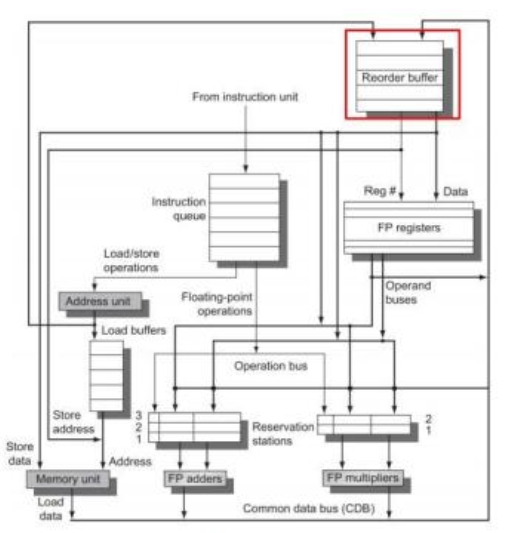
\includegraphics[width=0.7\linewidth]{Tomasulo_3.png}
    \caption{Speculative Tomasulo仿真器架构图}
    \label{fig: Real Toma}
\end{figure}

除了ROB,我们还可以看到以下部件:
\begin{enumerate}
    \item 指令队列(Instruction queue):存储待处理的指令。
    \item 浮点寄存器(FP registers):存储浮点数值的寄存器。
    \item 操作数总线(Operand bus):用于传送操作数至不同的功能单元。
    \item 浮点加法器(FP adders)和浮点乘法器(FP multipliers):执行浮点加法和乘法操作的功能单元。
    \item 保留站(Reservation stations):暂存那些已经分派但尚未执行的指令。
    \item 公共数据总线(CDB,Common Data Bus):功能单元用来将计算结果发送回重排序缓冲区或寄存器的总线。
    \item 地址单元和加载/存储缓冲区(Load/Store buffers):用于处理内存访问操作。
    \item 内存单元(Memory Unit)和地址单元(Address Unit)
\end{enumerate}

\section{代码实现}
我们按顺序实现以下部件:
\begin{enumerate}
    \item 重排序缓冲区(ROB)
    \item 公共数据总线(CDB,Common Data Bus)
    \item 保留站(Reservation stations)
    \item 地址单元和加载/存储缓冲区(Load/Store buffers)
    \item 浮点加法器(FP adders)和浮点乘法器(FP multipliers) 
    
\end{enumerate}

\subsection{额外假设}
我们假设指令加入buffer和从buffer删除也消耗一个周期
\subsection{ROB}
Reorder Buffer(ROB)有以下表项:\\

\begin{tabular}{|c|c|c|c|c|c|}
    \hline
    条目 & 繁忙 & 指令 & 状态 & 目的地 & 值 \\\hline
\end{tabular}
\\

因此我们定义如下的ROB类:
\begin{lstlisting}
    class Reorder_Buffer:
        class Buffer_Unit:
            def __init__(self, entry=0) -> None:
                self.entry = entry # 条目号
                self.busy = False  # 繁忙位
                self.instruction = []  # 指令
                self.states_name = None  # 状态
                self.states_num = [0, 0, 0, 0] #状态结束的周期
                self.destination = ''  # 目的地
                self.value = ''  # 值

            def display(self):  #显示自身状态
                print(f'entry{self.entry:<7}', end = ' : ')
                print(f'{"Yes" if self.busy else "No":<4}', end=', ')
                print(f'{str(self.instruction):<32}', end=', ')
                if self.states_name != None:
                    print(f'{self.states_name:<13}', end=', ')
\end{lstlisting}
\begin{lstlisting}[firstnumber=18]
                else:
                    print(' ' * 13, end=', ')
                print(f'{str(self.states_num):<17}', end=', ')
                print(f'{self.destination:<4}', end=', ')
                print(f'{str(self.value):<4}' + ';')

        def __init__(self,size=6):
            self.buffers = [self.Buffer_Unit(entry=i+1) for i in range(size)]
        def display(self):
            for unit in self.buffers:
                unit.display()
\end{lstlisting}
打印的位数是用 最长的可能位数+1计算的,数字按最多2位计。
打印测试如下图:
\begin{figure}[H]
    \centering
    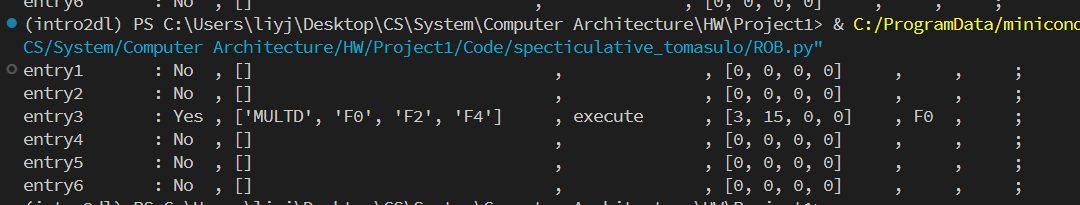
\includegraphics[width=\linewidth]{Tomasulo_4.png}
    \caption{ROG Display Test}
    \label{fig: ROB Disp_Test}
\end{figure}
\subsection{公共数据总线(CDB)}
\begin{lstlisting}
    class CDB:
        def __init__(self):
            self.data = 0
            self.source_entry = -1
\end{lstlisting}
模拟公共数据总线的类。\\
self.data:这个属性用来存储被传输的数据。在这个简化的模型中,data 被初始化为 0,表示最初没有数据在总线上。\\
self.source\_entry:这个属性用于标识产生 data 的源头(即数据来源的保留站的编号)。它被初始化为 -1,表示最初没有任何保留站向 CDB 发送数据。
\newpage
\subsection{保留站}
\begin{lstlisting}
    class Reservation_Station:
        def __init__(self, type="", id=0, CDB=None, ROB=None):
            self.type = type
            self.id = id
            self.busy = False
            self.Op = ''
            self.Vj = ''  # 拷贝可读取的数据
            self.Vk = ''
            self.Qj = ''  # 记录尚不能读取的数据将由哪条指令算出
            self.Qk = ''
            self.Dest = 0  # 目的ROB编号
            self.cdb = CDB
            self.rob = ROB

        def write_in(self):
            if self.busy == 'No':
                return
            if self.Qj == self.cdb.source_entry:
                self.Qj = ''
                self.Vj = copy.copy(self.cdb.data)
            if self.Qk == self.cdb.source_entry:
                self.Qk = ''
                self.Vk = copy.copy(self.cdb.data)

        def display(self):
            print(f'{self.type:<4}{self.id} : ', end= '')
            print(f'{"Yes" if self.busy else "No":<4}', end=', ')
            print(f'{self.Op:<8}', end=', ')
            print(f'{str(self.Vj):<30}', end=', ')
            print(f'{str(self.Vk):<30}', end=', ')
            print(f'{str(self.Qj):<3}', end=', ')
            print(f'{str(self.Qk):<3}', end=', ')
            print(f'{str(self.Dest):<4};')
\end{lstlisting}
根据PPT上的表项配置变量。\\
self.Qj 表示第一个源操作数所依赖的那个尚未完成的操作的保留站编号。
如果 self.Qj 等于 self.cdb.source\_entry,这意味着所依赖的操作已经完成,并且其结果已经在公共数据总线上可用。
self.Qj 被清空,表示不再依赖任何未完成的操作。\\
self.Vj 被设置为 self.cdb.data 的副本,这是因为 self.cdb.data 包含了所依赖操作的结果。这里使用 copy.copy 是为了确保 self.Vj 获得的是数据的副本,避免直接修改 self.cdb.data。
\\类似地,self.Qk 表示第二个源操作数所依赖的那个尚未完成的操作的保留站编号。




\subsection{地址单元和加载/存储缓冲区(Load/Store buffers)}
加法器和乘法器的实现基本类似,只需注意delay的区别(此处可以用一个flag位在每次执行时翻转,产生1的delay。但delay非1时不能这样做)

\begin{lstlisting}
    class Load_Buffer:
    class Load_Buffer_Unit(Reservation_Station):
        def __init__(self,type='load',id=0, CDB=None, ROB=None, register_states_=None):
            super().__init__(type=type,id=id,CDB=CDB,ROB=ROB)
            self.address = ''
            self.flag = 0
            self.register_states = register_states_


        def execute(self,cycle):
            if not self.busy:
                return
            rob_entry = self.rob.buffers[self.Dest]
            rob_entry.update_state(StateName.EXECUTE, 1)
            print(self.Qj,self.Qk)
            print(self.Qj,self.Qk)
            print(self.Qj, self.Qk)
            print(self.Qj, self.Qk)
            if self.Qj == '' and self.Qk == '' :
                self.address = self.Vj+self.Vk
                if self.Op == "LD" or (self.Op == "SD" and self.register_states[f'F{self.Dest+1}']=="No"):
                    self.flag = 1

    def __init__(self, CDB=None, ROB=None, register_states=None, memory=None, registers=None):
        self.buffers = [self.Load_Buffer_Unit(id=i, CDB=CDB,ROB=ROB,register_states_=register_states) for i in range(1,3)]
        self.head = 0
        self.memory = memory
        self.ROB = ROB
        self.CDB = CDB
        self.register_states = register_states
        self.registers = registers
        self.count=0
    def write_in(self):
        for i in range(2): self.buffers[i].write_in() 

    def execute(self,cycle):
        # print('cycle',cycle)
        if self.count==6: self.head = 1-self.head
        running_buffer = self.buffers[self.head]
        # flag标志位为1(表示地址计算已完成)
        #if running_buffer.Op == 'SD' and cycle >30 : running_buffer.flag = 1
        if running_buffer.flag:
            
            if running_buffer.Op == 'LD':
                #for i in range(CDB.source_entry):
                if running_buffer.Dest > self.CDB.source_entry:
                    '''
                    如果头部加载单元是一个加载指令 并且该指令的目的地小于通用数据总线(CDB)上当前的源指令索引,那么进行以下操作:
                    
                    从内存地址中读取数据并将其写入CDB
                    设置CDB的数据来源为当前加载单元的目的地
                    更新执行阶段结束的周期数
                    重新初始化当前加载单元并更新头部指针
                    '''
                    self.CDB.data = self.memory[running_buffer.address]
                    self.CDB.source_entry = running_buffer.Dest
                    

            elif running_buffer.Op == 'SD':
                temp = self.ROB.buffers[running_buffer.Dest].instruction[1]
                if type(temp) != int:
                    temp = self.registers[temp]
                self.memory[running_buffer.address] = temp
                self.ROB.buffers[running_buffer.Dest].value = 0

            self.ROB.buffers[running_buffer.Dest].states_num[1] = cycle
            running_buffer.__init__(id=running_buffer.id,CDB=self.CDB,ROB=self.ROB,register_states_=self.register_states)

            self.head = 1 - self.head 
            self.count+=1
        self.buffers[0].execute(cycle)
        self.buffers[1].execute(cycle)

    def display(self):
        self.buffers[0].display()
        self.buffers[1].display()

    def find_no_busy(self):
        for i in range(2):
            if not self.buffers[i].busy:
                return  i
        return -1
\end{lstlisting}

\subsection{主函数}
\begin{lstlisting}

    while top != bottom:
        # 逆序执行
        # 删除标记
        top, delete_sign, insert_sign = handle_delete_sign(
            rob, top, bottom, delete_sign, insert_sign)
        if top == None: break
        
        # commit
        delete_sign = commit(rob, top, registers, registers_name,
                             registers_state, result, delete_sign, cycle)
        
        
        # 写结果                  
        write_result(cdb, rob, loads, fp_adders, fp_multipliers, cycle)
        #执行
        loads.execute(cycle)
        fp_adders.execute(cycle)
        fp_multipliers.execute(cycle)

        # 发射
        top = issue_instructions(rob, top, bottom, loads, fp_adders,
                                 fp_multipliers, registers_name, registers_state, registers, cycle)
        
        line, bottom, insert_sign = handle_insert_sign(
            line, bottom, instructions, rob, insert_sign)

        display_status(cycle, rob, loads, fp_adders,
                       fp_multipliers, registers_name, registers_state)
        cycle += 1

    display_result(result=result)
\end{lstlisting}

处理删除标记(delete\_sign):
当 delete\_sign 为真时,重置位于 top 索引的重排序缓冲区(ROB)条目。
top 索引增加,以指向下一个条目。
重置 delete\_sign 并设置 insert\_sign,允许新的条目插入。
如果 top 和 bottom 相等,表示 ROB 为空,循环终止。\\
处理提交(commit):
如果 rob.buffers[top \% 6].value 不为空,表示该指令已经完成,可以提交。
更新寄存器值(除非是 SD 指令),释放相应资源。
将结果添加到 result 列表中,并准备删除该条目。\\
写结果(write\_result):
如果 cdb.source\_entry 不为 -1,表示 CDB 有数据可供写入。
更新相应的 ROB 条目,以及所有正在等待这个数据的保留站。\\
执行功能单元操作(execute\_units):
执行 loads, fp\_adders, fp\_multipliers 的 execute 方法。
处理发射指令(issue\_instructions):\\
遍历 ROB,寻找可以发射的指令。
如果找到,更新相关状态,并将指令分配给相应的功能单元。\\
处理插入标记(insert\_sign):
如果 insert\_sign 为真且还有未处理的指令,将新指令添加到 ROB 中。

\section{结果展示}
\begin{figure}[H]
    \centering
    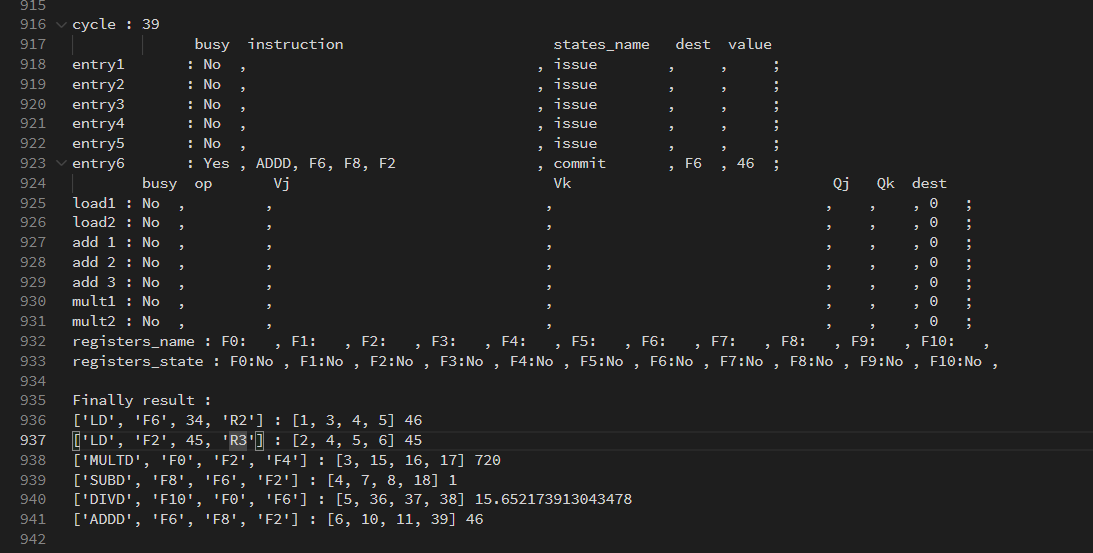
\includegraphics[width=\linewidth]{Output1.png}
    \caption{Output1}
    \label{fig: Output1}
\end{figure}


\begin{figure}[H]
    \centering
    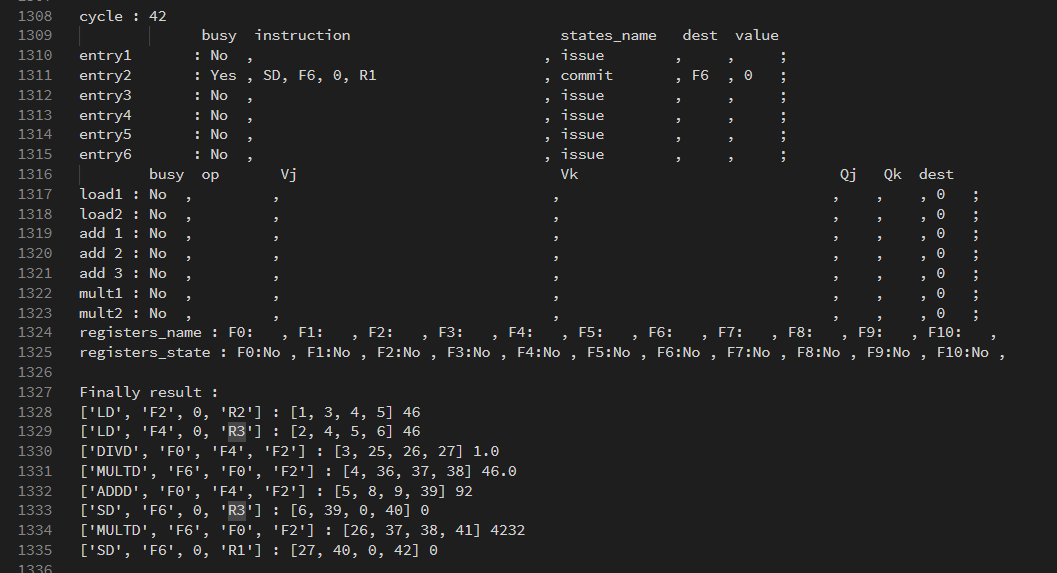
\includegraphics[width=\linewidth]{Output2.png}
    \caption{Output2}
    \label{fig: Output2}
\end{figure}

\newpage

\section{附加问题}

\subsection{Tomasulo 算法}
\begin{itemize}
  \item Tomasulo 算法的优点:
  \begin{itemize}
    \item 动态调度:可以在运行时动态地重新排序指令,减少数据冲突和结构冲突。
    \item 寄存器重命名:“写后写”和“读后写”冒险不是真冒险,没必要为他们阻塞指令的流动.通过重命名寄存器来减少 WAR 和 WAW 冲突。
    \item 更高的资源利用率:而且记分牌为了乱序执行指令,在碰到写后写、读后写这两个冒险的时候也会暂停流水线,而这其实是不必要的.由于Tomasulo动态调度和寄存器重命名,更有效地利用硬件资源。
    \item 适用于超标量架构:适合在一个周期内发射多条指令的处理器设计。
  \end{itemize}
  \item Tomasulo 算法的缺点:
  \begin{itemize}
    \item 硬件复杂性:实现 Tomasulo 算法需要更复杂的硬件支持。
    \item 功耗和成本:由于硬件复杂性,功耗和成本相比 Scoreboarding 更高。
    \item 每一个周期只能写回一条指令,还要增加额外的控制逻辑使得多条指令变得有序
    \item 存储指令之间也会发生数据冲突
    \item Tomasulo算法没办法实现精确中断
  \end{itemize}
\end{itemize}

\subsection{引入重排序缓冲区改进 Tomasulo 算法的原理}
重排序缓存的目的是让乱序执行的指令被顺序地提交.\\乱序提交是Tomasulo最大的缺点。
因为冯诺依曼结构向程序员承诺了处理器会按照程序的顺序来执行指令
,因此程序员在调试程序的时候会希望当他在某行代码停下来的时候,
代码前面的指令全部执行完,而代码后面的指令一条都没有执行,但是很显然,
一个乱序执行、乱序提交的机器是没办法达到程序员的预期的。
另外,因为控制指令、程序异常和外部中断也会截断指令流,
所以通过顺序提交指令来实现精确中断(这里的中断是指中断指令流)至关重要。\\
ROB的核心原理是记录下指令在程序中的顺序,
一条指令在执行完毕之后不会立马提交(这里的提交指的是修改处理器状态,如修改逻辑寄存器堆),
而是先在Buffer中等待,等到前面的所有指令都提交完毕,才可以提交结果到逻辑寄存器堆。

\subsection{重排序缓存的缺点}
\begin{itemize}
  \item 资源消耗:ROB 是一个大型的硬件结构,需要大量的寄存器和逻辑电路。
  \item 复杂的控制逻辑:管理 ROB 的逻辑非常复杂,特别是在处理分支预测失败和异常时。
  \item 限制了缓冲区大小:ROB 的大小是有限的,限制了可以乱序执行的指令数量。
  \item 潜在的性能瓶颈:如果 ROB 满了,新的指令无法被发射,可能导致性能下降。
\end{itemize}

\end{document}